\documentclass[t]{beamer}

\input{../basic-tex-config/preamble}

\usepackage{fontspec}
\setsansfont{ALSSchlangesans}

\usepackage{./beamer-itmo/beamer-itmo}

\uselanguage{russian}
\languagepath{russian}
\deftranslation[to=russian]{Theorem}{Теорема}
\deftranslation[to=russian]{Definition}{Определение}
\deftranslation[to=russian]{Definitions}{Определения}
\deftranslation[to=russian]{Corollary}{Следствие}
\deftranslation[to=russian]{Fact}{Факт}
\deftranslation[to=russian]{Example}{Пример}
\deftranslation[to=russian]{Examples}{Примеры}

\graphicspath{{../img/energy_loss/} {../img/}}

% Title

\title[Симп. мет. инт. ур-я Ландау-Лифшица]{Симплектические методы интегрирования\linebreak
    уравнения Ландау-Лифшица}
\author{Плотников Антон}
\date{Санкт-Петербург \today}

\begin{document}
\frame[plain]{\titlepage}

\begin{frame}
\frametitle{Магнитные скирмионы}
\framesubtitle{Введение}
    Скирмионы -- это топологически устойчивые вихревые структуры, наблюдаемые в
    магнитных решетках.

    \begin{figure}
        \centering
        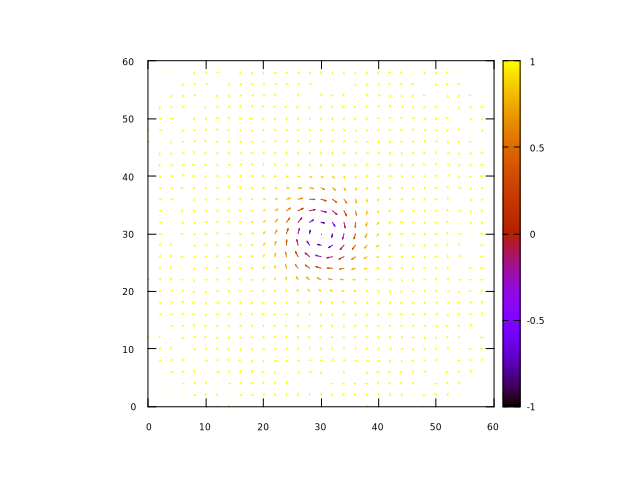
\includegraphics[scale=0.3]{../img/simple_skyrmion_1}
    \end{figure}
\end{frame}

\begin{frame}
    \frametitle{Магнитные скирмионы}
    \framesubtitle{Актуальность}
    Тема скирмионов сейчас весьма актуальна, за последний год скирмионы
    упоминаются более чем в 1000 статьях, по результатам поискового запроса в
    \url{schoolar.google.com}.

    В научных журналах рассматриваются возможности использования скирмионов в
    качестве эффективных ПЗУ за счет возможность потенциально высокой плотности
    размещения их на кристаллической решетке.
\end{frame}

\begin{frame}
\frametitle{Уравнение Ландау-Лифшица}
\framesubtitle{Постановка задачи}

Состояние магнитной системы описывается уравнением Ландау-Лифшица

\begin{block}{Уравнение Ландау-Лифшица}
\begin{align*}
    &\frac{dS_n}{dt} = -\gamma S_n \times H^{eff}_n - \gamma\lambda S_n \times
    \left(S_n\times H^{eff}_n \right)
    \\
    &H^{eff}_n = \nabla_{S_n}E = AS_n + B_n
\end{align*}
\end{block}
\end{frame}


\begin{frame}
    \frametitle{Постановка задачи}

    Большинство описанных моделей используют малоэффективные методы
    интегрирования, такие как метод Эйлера.


    \begin{columns}
        \begin{column}{0.3\textwidth}
            test
        \end{column}
        \begin{column}{0.7\textwidth}
            \vspace{4em}
            \centering
            \includegraphics[scale=0.3]{energy_loss_euler_1}
        \end{column}
    \end{columns}

    %Хотелось бы получить более
    %эффективный метод, который бы при этом сохранял энергию системы (если не
    %учитывать диссипативную часть уравнения Ландау-Лифшица), чтобы наблюдать
    %в динамике поведение скирмионов при изменении характеристик системы или
    %введении дополнительных источников снаружи.
\end{frame}

\begin{frame}
    \frametitle{Симплектический метод}
    В общем виде симплектический метод выдлядит следующим образом:

    \begin{block}{Общий вид симплектического интегратора}
        \begin{gather*}
            S_{n+1} = S_n + h\sum_{j=1}^s b_j f(t_n+c_jh, \xi_j)
            \\
            \xi_j = y_n + h\sum_{i=1}^{s}a_{ji} f(t_n+c_jh, \xi_i)
        \end{gather*}
    \end{block}
\end{frame}

\begin{frame}
    \frametitle{Метод ньютона}

\end{frame}

\end{document}
